\section{Linguaggi decidibili}
Obiettivi
\begin{itemize}
	\item Studiare il potere degli algoritmi
	\item Capire quali problemi sono risolvibili da un algoritmo e quali no
	\item In questa lezione iniziamo considerando problemi **decidibili** 
\end{itemize}

\subsection{Problemi sui linguaggi regolari}
\subsubsection{Problema dell'accettazione}
Ovvero, testare se un DFA accetta una stringa
$A_{DFA} = \{\langle B,w\rangle\mid B$  è un DFA che accetta la stringa $w\}$ 
$B$ accetta $w$ **se e solo se** $\langle B,w\rangle$ appartiene ad $A_{DFA}$ 
Mostrare che il linguaggio è **decidibile** equivale a mostrare che il problema computazionale è**decidibile**. 

\begin{theorem}{$A_{DFA}$ è decidibile}\end{theorem}
\g{Idea}: definire una TM che decide $A_{DFA}$ 
$M=$ "Su input $\langle B,w\rangle$, dove $B$ è un DFA e $w$ una stringa: 
\begin{enumerate}
	\item Simula $B$ su input $w$ 
	\item Se la simulazione termina in uno stato finale, \g{accetta}. Se termina in uno stato non finale, \textit{rifiuta}."
\end{enumerate}
	

\paragraph{Dimostrazione}
\begin{itemize}
	\item la codifica di $B$ è una lista dei componenti: $Q,\Sigma,\delta, q_0$ e $F$ 
	\item fare la simulazione è facile
\end{itemize}


\begin{theorem}{$A_{NFA}$ è decidibile}\end{theorem}
$A_{NFA} = \{\langle B,w\rangle\mid B$ è un $\varepsilon$-NFA che accetta la strina $w\}$ 
\g{Idea}: usiamo la TM $M$ che decide $A_{DFA}$ come subroutine.

\g{Dimostrazione}: 
$N=$ ``Su input $\langle B,w\rangle$, dove $B$ è un $\varepsilon$-NFA e $w$ una stringa: 
\begin{enumerate}
	\item Trasforma $B$ in un DFA equivalente $C$ usando la costruzione per sottoinsiemi
	\item Esegui $M$ con input $\langle C,w\rangle$ 
	\item  Se $M$ accetta, \g{accetta}; altrimenti, \textit{rifiuta}.''
\end{enumerate}
$N$ è un decisore per $A_{NFA}$, quindi $A_{NFA}$ è **decidibile**. 

\begin{theorem}$A_{REX}$ è decidibile\end{theorem}
$A_{REX} = \{\langle R, w\rangle\mid R$ è una espressione regolare che genera la stringa $w$ $\}$ 
\g{Idea}: usiamo la TM $N$ che decide $A_{NFA}$ come subroutine

\b{Dimostrazione}:
$P=$ ``Su input $\langle R,w\rangle$, dove $R$ è una espressione regolare e $w$ una stringa: 
\begin{enumerate}
	\item Trasforma $R $in un $\varepsilon$-NFA equivalente $C$ usando la procedura di conversione
	\item  Esegui $N$ con input $\langle C,w\rangle$ 
	\item  Se $N$ accetta, \g{accetta}; altrimenti \textit{rifiuta}.''
\end{enumerate}
$P$ è un decisore per $A_{REX}$, quindi $A_{REX}$ è \g{decidibile} 

\g{Riassumendo}
\begin{itemize}
	\item Ai fini della **decidibilità**, è equivalente dare in input alla TM un DFA, un $\varepsilon$-NFA o una espressione regolare
	\item La TM è in grado di con ertire una odifica nell'altra
	\item \g{Ricorda}: mostrare che il linguaggio è \g{decidibile} equivale a mostrare che il problema computazionale è \g{decidibile}.
\end{itemize}

\subsection{Test del vuoto}
Negli esempi precedenti dovevamo decidere se una stringa appartenesse o no ad un linguaggio.
Ora vogliamo determinare se un automa finito accetta una \g{qualche} stringa
$E_{DFA}=\{\angle A\rangle\mid A$ è un DFA e $L(A)=\varnothing\}$ 
Puoi descrivere un algoritmo per eseguire questo test? 

\subsection{$E_{DFA}$ è decidibile}
\g{Dimostrazione}: verifica se c'è uno stato finale che può essere raggiunto a partire dallo stato iniziale. 
$T=$ ``Su input $\langle A\rangle$, la codifica di un DFA $A$: 
\begin{itemize}
	\item \g{Marca} lo stato iniziale di $A$. 
	\item \g{Ripeti} la fase seguente fino a quando non vengono marcati nuovi stati: 
	\item \g{marca} ogni stato di $A$ che ha una transizione proveniente da uno stato già marcato
	\item Se nessuno degli stati finali è marcato, \g{accetta}; altrimenti \textit{rifiuta}.''
\end{itemize}

\subsection{Test di equivalenza}
$EQ_{DFA} = \{\langle A,B\mid A$ e $B$ sono DFA e $L(A)=L(B)\}$ 
\g{Idea}: 
\begin{itemize}
	\item costruiamo una DFA $C$ che accetta solo le stringhe che sono accettate da $A$ o da $B$, ma non da entrambi
	\item se $L(A)=L(B)$ allora $C$ non accetterà nulla
	\item il linguaggio di $C$ è la \g{differenza simmetrica} di $A$ e $B$ 
\end{itemize}

\subsection{$EQ_{DFA}$ è decidibile}
\g{Dimostrazione}: 
\begin{itemize}
	\item la \g{differenza simmetrica} di $A$ e $B$ è 
  	$L(C)= \Big( L(A)\cap \overline{L(B)}\Big) \cup \Big(\overline{L(A)}\cap L(B)\Big)$ 
	\item i linguaggi regolari sono \g{chiusi} per unione, intersezione e complementazione
	\item $F=$ ``Su input $\langle A,B \rangle$ dove $A$ e $B$ sono DFA: 
		\begin{enumerate}
			\item Costruisci il DFA $C$ per differenza simmetrica
			\item Esegui $T$, la TM che decide $E_{DFA}$ con input $\langle C\rangle$ 
			\item Se $T$ accetta, \g{accetta}; altrimenti \textit{rifiuta}.''
		\end{enumerate}
\end{itemize}

\subsection{Problemi per linguaggi Context-free}
$A_{CFG} = \{\langle G,w\rangle\mid G$ è una CFG che genera la stringa $w\}$ \\
\g{Idea}: costruiamo una TM che provi tutte le derivazioni di $G$ per trovarne una che genera $w$ \\
\g{Perché questa strategia non funziona?}

\subsection{$A_{CFG}$ è decidibile}
Se la CFG è in forma normale di Chomsky, allora ogni derivazione di $w$ è lunga \g{esattamente} $(2|w| -1)$ \g{passi}.\\
Le TM possono convertire le grammatiche nella forma normale di Chomsky!

\g{Dimostrazione}:
$S=$ ``Su input $\langle G,w\rangle$, dove $G$ è una CFG è $w$ una striga:
\begin{enumerate}
	\item Converti $G$ in forma normale di Chomsky
	\item Elenca tutte le derivazioni di $2|w|-1$ passi. Se $|w| = 0$, elenca tutte le derivazioni di lunghezza 1
	\item Se una delle derivazioni genera $w$, \g{accetta}; altrimenti \textit{rifiuta}."
\end{enumerate}

\subsection{Test del vuoto}
$E_{CFG}=\{\langle G\rangle\mid A$ è una CFG ed $L(G)=\varnothing\}$ 
\begin{itemize}
	\item \g{Problema}: non possiamo usare $S$ del teorema precedente. \g{Perché no?}
	\item Bisogna procedere in modo diverso!
\end{itemize}
\g{Idea}: stabilisci per ogni variabile se è in grado di generare una stringa di terminali

$R=$ ``Su input $\langle G\rangle$, la codifica di una CFG $G$: 
\begin{enumerate}
	\item \g{Marca} tutti i simboli terminali di $G$
	\item \g{Ripeti} la fase seguente fino a quando non vengono marcate nuove variabili: 
	\item \g{Marca} ogni variabile $A$ tale che esiste una regola $A\rightarrow U_1\dots U_k$ dove ogni simbolo $U_1\dots U_k$ è già stato marcato. 
	\item Se la variabile iniziale non è marcata, \g{accetta}; altrimenti \textit{rifiuta}.''
\end{enumerate}

\begin{theorem}
	$EQ_{CFG}$ è decidibile
\end{theorem}
$EQ_{CFG} = \{\langle G,H\mid G$ e $H$ sono CFG e $L(G)= L(H)\}$ 
\g{Idea}:
\begin{itemize}
	\item Usiamo la stessa tenica di $EQ_{DFA}$ 
	\item Calcoliamo la \g{differenza simmetrica} di $G$ e $H$ per provare l'equivalenza
\end{itemize}

\begin{center}
	{\Large STOP!}
\end{center}
\begin{itemize}
	\item Le CFG non sono chiuse per complementazione ed intersezione
	\item $EQ_{CFG}$ \g{non è decidibile!}
\end{itemize}

\subsection{Relazioni tra classi di linguaggi}
\begin{theorem}
	ogni CFL è decidibile
\end{theorem}
\g{Domanda}:
\begin{itemize}
	\item è facile simulare la pila con una TM
	\item sappiamo che le TM nondeterministiche possono essere simulate da una TM deterministica
\end{itemize}
\g{Non basta semplicemente simulare un PDA con una TM?}\\
Quali altre opzioni abbiamo? 

\begin{itemize}
	\item Dato un CFG $L$, sia $G$ la grammatica per $L$ 
	\item Costruiamo la TM $S$ che decide $A_{CFG}$ 
	\item La TM che decide $L$ è \\
  	$M_G=$ "Su input $w$: 
		\begin{enumerate}
	  	\item Esegui la TM $S$ con un input $\langle G, w\rangle$ 
	  	\item se $S$ accetta, \g{accetta}; altrimenti, \textit{rifiuta}
		\end{enumerate}
\end{itemize}


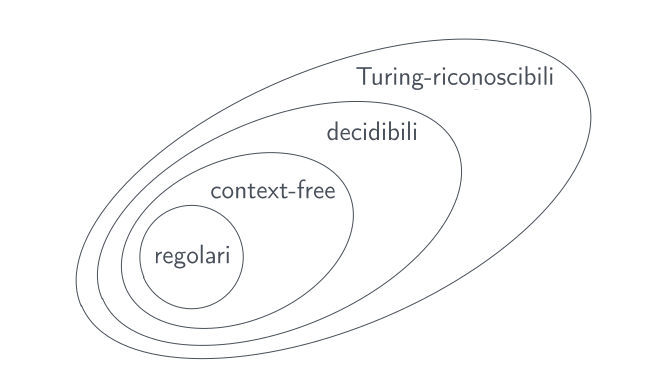
\includegraphics[scale=0.5]{img/rel_classi_linguaggi.png}
Queste non sono solo classi di linguaggi, ma anche \g{classi di capacità computazionale}. 
